\documentclass[11pt]{article}






\usepackage[utf8]{inputenc} % encode en UTF8

\usepackage[T1]{fontenc}





\usepackage[top=2cm, bottom=2cm, left=3cm, right=3cm]{geometry}
\usepackage{graphicx}
\usepackage{caption}
\usepackage{subcaption}
\usepackage{float}
\graphicspath{ {./photo/} }

%Belles fraction de fration \cfrac
\usepackage{amsmath}

\usepackage{tikz}
\usepackage{circuitikz}




\newcommand{\HRule}{\rule{\linewidth}{0.5mm}} % Epaisseur des lignes horizontales

\pagestyle{empty}
\newcommand{\myTitle[1]}{
\begin{minipage}{.47\textwidth}
\centering
\begin{flushleft}

\includegraphics[width=0.75\textwidth]{./photo/nantes_universite_logo.png}
\end{flushleft}
\end{minipage}
\begin{minipage}{.47\textwidth}
\centering
\begin{flushright}
\hspace*{1cm} 
\includegraphics[width=0.85\textwidth]{./photo/logo_polytech_nantes}
\end{flushright}
\end{minipage}~\\[1.5cm]

\begin{center}
\vspace*{\stretch{0.3}}
\end{center}

\begin{center}
  \Large
  \vspace*{\stretch{1}}
  \HRule \\[0.2cm]
  \begin{center}
    \huge
    \textbf{#1}\\ %Titre
  \end{center}
  %\textbf{\\ Projet Transversal}\\ %matière
  \HRule \\[1.5cm]
  
%  \vspace*{\stretch{5}}
%  
%  \small
%  \noindent Rédigé par \\
%  \vspace*{\stretch{0.2}}
%  \large
%  \noindent \Redac\\
%  \vspace*{\stretch{0.5}}
 
\end{center}

\vspace*{\stretch{2}}

\begin{center}\large
	\textsc{École Polytech de Nantes}\\
	\textsc{Département Électronique et Technologie du Numérique}
\end{center}

\vspace*{\stretch{5}}

\begin{center}
	\begin{minipage}{0.4\textwidth}
		\begin{flushleft} \large
        	\noindent Rédigé par\\ %\Redac
			Victor DUFRENE \\
			Mathis BRIARD\\
			Louison GOUY\\
			Yujie HUANG
		\end{flushleft}
	\end{minipage}
	\begin{minipage}{0.4\textwidth}
		\begin{flushright}\large
			Professeur encadrant : \\Yann MAHE\\ Anne CHOUSSEAUD\\
						
		\end{flushright}
	\end{minipage}
\end{center}
}

\begin{document}
\myTitle[Rapport de mini-projet \\ - Électronique Hautes Fréquences - ]
\newpage

\section{Résumé}


\newpage

\section{Synthèse de filtre passe-bas en technologie }


L'objectif est de réaliser un filtre passe-bas dont le gabarit est donné à la figure \ref{fig:gabarit_PB} avec une réponse de Tchebychev.

\begin{figure}[H]
	\centering
	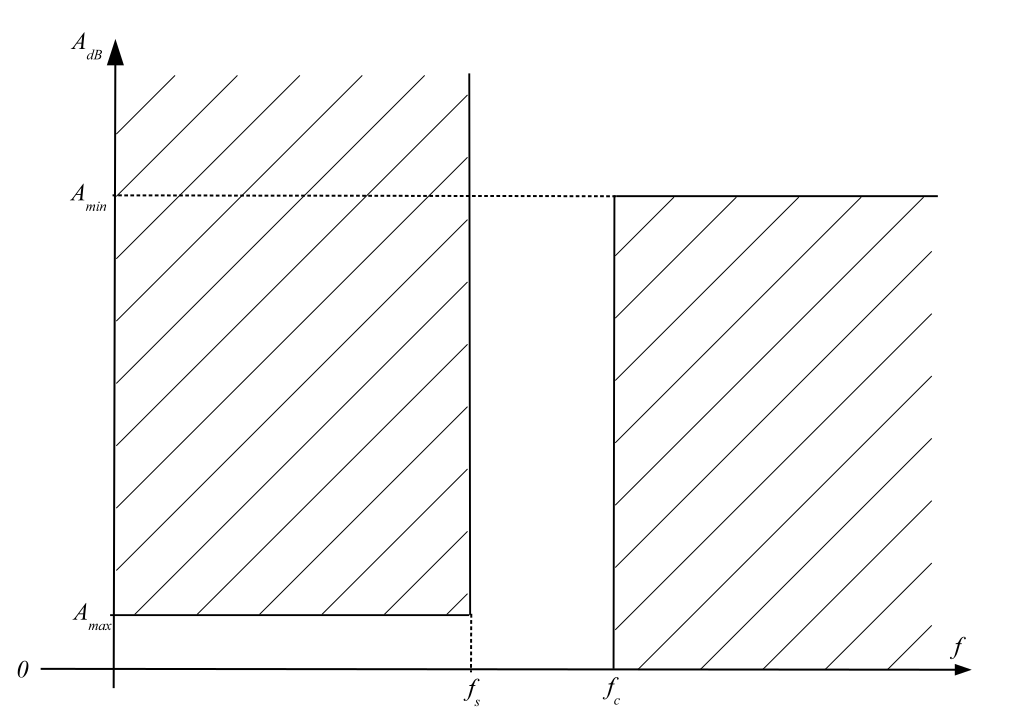
\includegraphics[width=15cm]{photo/gabarit_PB.png}
	\caption{Architecture de la balise}
	\label{fig:gabarit_PB}
\end{figure}


La conception d'un filtre hautes fréquences débute par une synthèse classique avec des éléments passifs (condensateurs et bobines) comme il a été fait dans le module moyennes fréquences du S7. A partir du gabarit de la figure \ref{fig:gabarit_PB}, l'équation ci-dessous nous est permet d'obtenir l'ordre du filtre à concevoir.



\begin{equation}
	n \geq \frac{argch(\sqrt{\frac{\alpha_{min}-1}{\alpha_{max} -1}})}{argch(1/k)}
\end{equation}


Où :
\begin{itemize}
	\item n est l'ordre du filtre souhaité;
	\item k est la sélectivité égal à$\frac{fc}{1,5fc} = \frac{2}{3} \approx 0,67$;
	\item $\alpha_{min}$ est l'atténuation minimale (en linéaire) du signal dans la bande atténué égal à $10^{\frac{15}{10}} \approx 31,6$
	\item $\alpha_{max}$ est l'atténuation maximale (en linéaire) du signal dans la bande passante égal à $10^{\frac{0,1}{10}} \approx 1,02$
\end{itemize}

Ce qui nous donne une application numérique où $n \geq 4,5$ ce qui nous donne un ordre 5 minimum pour respecter le gabarit souhaité.

%\begin{circuitikz}
%	\draw (0,0) to [R,v=$U_1$] (2,0);
%\end{circuitikz}
\begin{figure}[H]
	\centering
	\begin{circuitikz}
		\draw (0,0)
		to[V,v=$U_e$] (0,2) % The voltage source
		to[L=$l_1$] (2,2)
		to[C=$c_2$] (2,0) % The resistor
		(2,2)to[L=$l_3$] (4,2)
		to[C=$c_2$] (4,0) % The resistor
		(4,2)to[L=$l_3$] (6,2)
		to [R=$r$] (6,0) 
		to[short] (0,0);
	\end{circuitikz}
	\caption{Schéma prototype d'un filtre passe-bas de Tchebycheff en impédance.}
\end{figure}




\end{document}